\documentclass[11pt]{article}
\usepackage{fullpage}
\usepackage{tikz}
\PassOptionsToPackage{hyphens}{url}\usepackage{hyperref}
\usepackage{wrapfig}


\usetikzlibrary{shapes.geometric, arrows}

\tikzstyle{file} = [rectangle, rounded corners, minimum width=3cm, minimum height=1cm, text centered, text width=3cm, draw=black]
\tikzstyle{fileL} = [rectangle, rounded corners, minimum width=3cm, minimum height=1cm, text centered, text width=4cm, draw=black]
\tikzstyle{folder} = [rectangle, minimum width=3cm, minimum height=1cm, text centered, text width=3cm, draw=black]
\tikzstyle{arrow} = [thick, ->, >=stealth]

\begin{document}

\title{\vspace{-2cm}Final Report - Group 16}
\author{Ayoob Ahmed, Aayush Dalal, Al-Maz Ahmad, Devam Savjani}


\maketitle
\section{Introduction}
This report goes through our group project on the ARM 11 assembler, our extension which is extreme tic tac toe. For our implementation of the ARM 11 emulator, see {\tt{doc/Checkpoint.pdf}}. We have also included our group analysis as well as our individual evaluations.

\section{Structure and implementation of Assembler}
We approached coding the assembler in a structured manner, as suggested by the spec. We decided to use the two-pass strategy since everyone in our group found it easier to understand compared to only having a single pass. In our {\tt{firstPass}}, we stored the labels and their memory addresses in a symbol table whilst also storing each line as a string in an array of strings to assist the second pass. In the second pass, we read each line from the array of strings which was previously initialised, split up the instruction in terms of its mnemonic and operands and passed the split up instruction into its respective function (e.g. 'mov' was passed to a data process function).
\\Before writing in the binary file we need to do some preprocessing, to do this we convert the instruction from big-endian form to little-endian form. To write the values into a binary file we separate the 32-bit little-endian integer into 4 8 bit integer values and then write each 8-bit value into a binary file.
\\ We created an {\tt{assembler\_utils}} directory which that contains the file for all constants and files for each instruction. The structure of our assembler is as follows:

\begin{itemize}
	\item {\tt{assemble.h}} and {\tt{assemble.c}} - {\tt{assemble.c}} contains the c code that is at the top layer of the assembler, this file functions from the other files in {\tt{assembler\_utils}}. Inside the {\tt{assemble.c}} file, we ensure that the arguments are passed correctly, we call functions to process the file into a format our c program can manipulate (an array of instructions), we complete the first pass in this file and then convert each instruction into its binary equivalent using the helper functions. The file also ensures the instructions are in the correct endian format before writing to the binary file, and it finally writes the converted instructions to the binary file.
    The assemble.h file contains the structure for the table which stores the value for the results of the first pass, it also stores the enums for all of the different types of mnemonics and the declaration of all the functions used in the {\tt{assemble.c}} file.
	
	\item {\tt{mnemonicHelper.c}} - is the c program file that contains a function which returns the mnemonic of an instruction. The mnemonics are stored as enum values in the {\tt{assemble.h}}.
	
	\item {\tt{processBranch.c}}, {\tt{processDP.c}}, {\tt{processLSL.c}}, {\tt{processMul.c}} and {\tt{processSpecial.c}} - these files contain appropriate files that convert an array of strings (the instructions) into a 32-bit integer which is the binary equivalent. These files require helper functions which are included from the {\tt{processHelpers.c}} file.
	\item {\tt{processHelpers.c}} - these provide helper functions for {\tt{assemble.c}} as well as the process files as mentioned previously.
	
\end{itemize}


\begin{center}

\scalebox{0.8}{
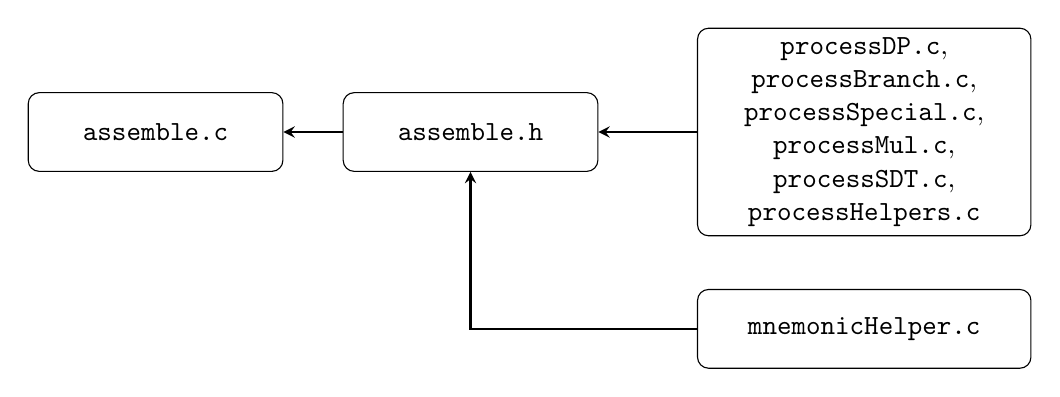
\begin{tikzpicture}[node distance=1cm]
\node (assembleC) [file] {{\tt{assemble.c}}};
\node (assembleH) [file, right of=assembleC, xshift=3cm] {{\tt{assemble.h}}};
\node (processes) [fileL, right of=assembleH, xshift=4cm] {{{\tt{processDP.c}}, {\tt{processBranch.c}}, {\tt{processSpecial.c}}, {\tt{processMul.c}}, {\tt{processSDT.c}}}, {{\tt{processHelpers.c}}}};
\node (mnemonicHelper) [fileL, below of=processes, yshift=-1.5cm] {{\tt{mnemonicHelper.c}}};

\draw [arrow] (assembleH) -- (assembleC);
\draw [arrow] (mnemonicHelper) -- ++(-5,0) -| (assembleH);
\draw [arrow] (processes) -- (assembleH);

\end{tikzpicture}}
\end{center}

We also handle the optional test cases in a way such that the operands can be of either type, i.e. r1 lsl \#1 or r1 lsl r2. We accomplished this by using the {\tt{getInt}} function on the first element of the operand. If operand has a shift then it uses {\tt{getShiftAmount}} function to convert the shift into binary.

\section{Extension}
\subsection{Introduction}
Our extension was an implementation of the game Extreme Tic Tac Toe and an AI to play the game. Firstly, we will discuss the structure of the game and how we implemented it and then we will discuss how the AI works.
\\Extreme Tic Tac Toe is a variation of the normal game where each cell is its own tic tac toe game. When a player plays in a "box" within a cell the next player will have to play in the cell which is numbered the same as the box within the cell. So for example, if player 1 plays in the middle box in cell number 0 (the cells are numbered from 0 in the top left to 8 in the bottom right), then player 2 will have to play in the top left cell. If this cell has already been won or the cell is full, then the next player will have a free pick of their cell and position and the game will continue from there. The game ends when either the board is full or one player has won a row of cells.
\subsection{Our Implementation}
\subsubsection{Board Representation}
We represented the board as 3 arrays of cells with each array representing one row of cells. Each cell was then 3 arrays of integers. We could have potentially used arrays of chars but we felt that it was easier to work out if the game was finished if we used integers. Each cell also had a corresponding cell which is an enum where the options are AIWIN, PLAYERWIN, DRAW or TBD. This was updated when a cell was played in.

\subsubsection{The Algorithm and our Tweaks}
The minimax algorithm works by simulating all possible plays from both players from a certain game state until either the game is finished or the game is completed. Then an evaluation function is used to give a score to the game state, as shown in Figure 1. In the cases where we are simulating the AI playing, it will choose the play that has the highest value and vice versa for when we are simulating the player playing. These scores will propagate up the tree and eventually each play that the AI can take from the original game state will have a score and the AI will pick the play with the highest score.
\\\\Since there were two types of plays (for extreme tic tac toe), a restricted pick and a free pick we created a minimax function for each type which could call each other depending on if the {\tt{gameState}} required it. In the normal game of tic tac toe, since there are not many possible {\tt{gameState}}s (in comparison to extreme tic tac toe), the AI can see all potential paths and make the most informed guess and therefore it is not possible to beat an AI using a well-implemented minimax algorithm playing tic tac toe. As the algorithm covers all possibilities, we can say that its maximum depth is 100\% of the possible depth and we can also say that the maximum depth is the same as how "good" the AI is playing the game so it is important to try and have this depth as high as possible. Despite this, we attempted to implement a simple minimax algorithm that would recurse until it hit a state where the game was won however as expected, the computer took too long to compute the move.

\begin{wrapfigure}{r}{0.4\textwidth}
	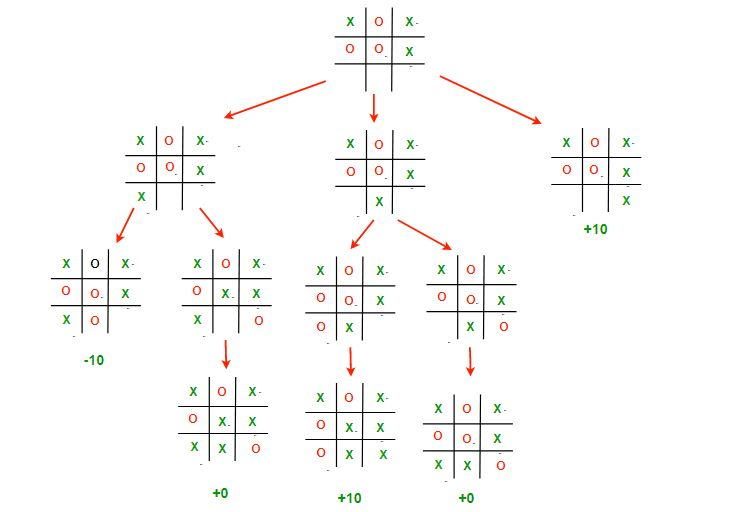
\includegraphics[scale = 0.5]{minimax.jpeg}
	\caption{A Visual representation of the algorithm - image from \url{https://www.geeksforgeeks.org/minimax-algorithm-in-game-theory-set-3-tic-tac-toe-ai-finding-optimal-move/}}
\end{wrapfigure}

We then implemented a maximum depth for the algorithm and at that depth, it would just calculate the "score" of the board (how good the board is for the AI) and try to propagate that score up the table. In the beginning, this depth was very small since we had not optimised the algorithm. We added alpha beta pruning to try and remove paths that would not be chosen by adding two integer parameters to both functions, alpha and beta. Alpha would be set to a small number and beta would be set to a large one. Alpha would only be updated in the case where we were trying to find the largest score (simulating the AI playing) and then it would be the maximum of the score calculated from minimax and itself. Beta is calculated similarly but from the minimum of the minimax value from when we simulate the player playing and itself. If at any point alpha is smaller than beta we break the loop since this path will not be optimal since either the score is too small for the AI to pick or the score is too big for the simulated player to pick. This cut out quite a few branches and allowed us to increase the depth and therefore make the AI smarter. The largest increase came from using a new technique. In both minimax algorithms, we would go through all possible moves and call minimax on the state that they lead to. With our optimisation, we made the AI either simulate a player play or AI play (depending on if we wanted to find the minimum score or maximum score respectively) and then we calculated score of the cell (or board if it was a free pick) and put it in an array of {\tt{potentialPath}}s where each {\tt{potentialPath}} had the position (and cell if it was a free pick) and the corresponding score. We then sorted them by ascending order if we were in the maximising case (the AI) and vice versa for the minimising case. We also counted how many potential paths there were and we only recursively called minimax on the top half. This let us weed out any sub-optimal moves and let us focus in on the moves that would lead to victory. Since we were shaving off sub-optimal moves at every level the maximum depth that we could achieve was increased greatly and this made our AI smarter and more difficult to play against.
\subsubsection{Functions}
As previously mentioned, there are two types of situations, a free pick and a restricted pick, hence we created two functions, {\tt{minimaxFree()}} and {\tt{minimaxRestricted()}}, for writing to the table. They both check if the inputs are out of bounds and if the target box has already been written to and if so ask the player to write to them again. The important thing that they both have in common is an integer pointer parameter. This holds the position within the cell that the player chose to play in so that the next player can play in the corresponding cell. They both have a boolean in their parameters called {\tt{isPlayer}} and this is used in the actual writing process to see if either a 1 (which represents a player and in the textual representation of the board gets converted to an X) or a 2 (which represents the AI and gets converted into an O).
The game continues until either there are no more places to play in or the game is won.
\\\\We had two evaluation functions, one was a function that evaluated the whole board and another evaluated just a cell. The function that evaluated the board just added up all the cell evaluations. The one that evaluated a single cell would start off by seeing if the cell had been won already. If so it would immediately return the value (-10 for a player win and 10 for an AI win). If not it would then try to calculate how many two-in-a-rows that could be finished. It would do that for both the player and the AI. Then it would see how many AI plays and player plays were in the power positions. These were the middle and the corners (the middle was more valuable than the corners) as they are the most important places to secure in order to win. We would add for any times the AI had a play in these positions and subtract any time the player had a play in these positions. In the end, we would add the AI pairs and subtract the player pairs and add the power positions total to get the score of the cell. This incentivised the AI to pursue the middle and then securing 3-in-a-rows to win the game.
We also had a function that would print the table to the terminal. The function begins by creating an array of strings, of which each string has 21 characters and the string array has a length of 9. It then writes each row to a string and then prints them in order with a gaps between them.
\subsection{Testing}
In terms of testing our program, initially stepping through gdb and ensuring each function works as expected. We went through all edge cases we could think of and then ensured that the edge cases were handled correctly. In this way, we were able to feel confident that our functions were working.
\\After testing individual functions, we then set on testing all the functions after they were all stringed together by playing the game countless times to ensure the game works. Furthermore, we got other people to play the game as playing the game with fresh eyes would enable the testing of the game more exhaustive. Hence by using this tactic, we can say that we are confident that the game works.

\section{Group Reflection}
In terms of our group dynamic and how we have worked as a team for the assembler, we believe it has been a huge success. Learning from our mistakes in the emulator, we decided to stick to our strategy of communicating on discord calls daily. Furthermore, we carried on updating logs on discord and this was extremely helpful, especially when the two members who had been debugging the emulator returned. Adhering to our implemented strategy ensured that we finished the code from the assembler much quicker and without any major setbacks. If someone was unsure about their task, we swapped tasks between that member and another member who understands the problem to find a working solution efficiently. In addition to this, we also decided that if someone finishes implementing their function, they will help another member by looking at the discord logs and picking the member with the least progress. Once everyone was finished doing their part of the code, similar to the emulator, we decided to assign two people to combine the implemented functions together. The other two began working on the remaining part of the project (the extension). After splitting up into two groups, the group working on the assembler completed the debugging and testing of the code. They implemented code to pass the optional tests and after passing all required (and optional) tests, they attempted to make the program more efficient while getting rid of any unnecessary code.

\subsection{Individual Relections}
\subsubsection{Al-Maz Ahmad}
My group was very welcoming and determined to finish the task as soon as possible. We would regularly meet on discord or talk over WhatsApp updating everyone about the current status of the project. They were all very hardworking and I quickly noticed that if someone were falling behind or struggling, we would work as a team and delegate someone to help. For example, towards the end of the assembler, my debugging tools stopped working, so it made it very difficult to locate bugs or test my program, Devam stepped in and we began testing the code together, bouncing ideas off of each other identifying things the other could not. I also noticed that I was able to listen to the team, complete tasks that were delegated, and provide useful ideas when analysing our approach. I think my main weakness is debugging, up until the last few weeks of the project my debugging methods were not effective taking up more time then I had hoped. After asking my team for some advice I was pointed in the right direction of a virtual machine, which provided easy access to the appropriate debugging tools. For future group projects, I think I will try to be more aware of errors that might present themselves by implementing more edge case tests.
\subsubsection{Ayoob Ahmed}
I felt that I fit well into the group. I thought that one of my strengths was organising the group. For example, it was my idea to split the group in half towards the end of development on the emulator and have two of us begin work on the assembler. I thought that this was very effective as we began work on the assembler earlier and it let half the group become more comfortable with the inner workings of the assembler so when the rest of the group caught up they could help get them up to speed. Also, having new people join the group did have an opportunity to have new ways of solving problems that were plaguing the first group. I think that my main weakness was applying bad overall structures to the programs. We spent a couple of days working on using integer arrays of length 32 to represent the memory and registers of the processor. This was a bad idea because it took up a lot of memory and was extremely clunky. I think in the future I will plan out my ideas for longer and try to find any weaknesses in them.
\subsubsection{Aayush Dalal}
As a group, I think we all were great. We tried to split the work evenly between every group member from the beginning and in my opinion, every member did their part in a thorough manner and within the required time. I found the discord calls and logs helpful as they gave me an idea of where everyone was at. This was particularly helpful when I was stuck while implementing a function in the emulator. Since I knew that Ayoob had finished his function (through the logs), I was able to ask him for help. In terms of my contribution to the group, I think my most helpful contribution was debugging and testing the code as this ensured that we passed all the required tests and also gave me a better understanding of how everyone went about implementing their functions. However, one thing I would like to improve on is my availability. Even though we had planned times for meetings/discord calls, I sometimes ended up forgetting about them or was unavailable at the time as other work had come up. In the future, I would like to be able to plan my schedule better so this does not occur.
\subsubsection{Devam Savjani}
In terms of fitting in the group, I don’t think it was a worry as I knew the majority of the team prior to the project and I was able to bond with the other members, that I had not met before, very well. In constant communication with each other further developed our group dynamic and relationship with each other. Hence I believe the overall fit of the group was very good. I believed that our group approached the project with a high level of determination and also pulled through as well, with all of us putting a lot of effort in the project, which is also evident with all of our DocPA scores.
In terms of my strengths with the project, I believe one of my major strength was communication as especially during the first week, we were a bit lost and all a bit confused I believe communicating with each individual within the team gave the project a good boost, as after I had let everyone know what to do and split the tasks up more explicitly, we were making good progress. Another one of my strengths, I think also made the project go more smoothly was debugging and helping others debug was key to the success of our project.
\\Regarding my weaknesses, I believe one of my weaknesses was definitely my use of git, as I had never worked on a group project using git before therefore branching and merging were definitely new things, however, the decision for us all to learn how to use it before we started working was very helpful. Along with some help from Ayoob, I am now comfortable using git in a group project.
\\Another thing I think I would need to improve is organising the team meetings and understanding team members schedule better as there were times where team members were busy and were unable to work which definitely made organising the meetings better, however having the system on discord to log updates was definitely helpful for all of us.
\\If I was placed in another team, I believe my approach to organising the team and communicating would better an efficient way to handle the team, however as previously mentioned I would try to get a better understanding on how everyone works earlier on in the project.

\end{document}
